\documentclass{article}
\usepackage[preprint]{neurips_2025}
\usepackage[utf8]{inputenc} % allow utf-8 input
\usepackage[T1]{fontenc}    % use 8-bit T1 fonts
\usepackage{hyperref}       % hyperlinks
\usepackage{url}            % simple URL typesetting
\usepackage{booktabs}       % professional-quality tables
\usepackage{amsfonts}       % blackboard math symbols
\usepackage{nicefrac}       % compact symbols for 1/2, etc.
\usepackage{microtype}      % microtypography
\usepackage{xcolor}         % colors
\usepackage{amsmath}
\usepackage{cleveref}
\usepackage{commath}
\usepackage{graphicx}
\title{Gauss-Newton under adversarial attacks}


% The \author macro works with any number of authors. There are two commands
% used to separate the names and addresses of multiple authors: \And and \AND.
%
% Using \And between authors leaves it to LaTeX to determine where to break the
% lines. Using \AND forces a line break at that point. So, if LaTeX puts 3 of 4
% authors names on the first line, and the last on the second line, try using
% \AND instead of \And before the third author name.


\author{%
    Marshall Jiang \\
    \texttt{marshall.jiang@gmail.com} \\
}


\begin{document}


    \maketitle


    \begin{abstract}
        The use of gradient-only optimizer is considered standard in training deep neural networks due to its flexibility and speed.
        However, there has been interest in using Hessian information in accelerating gradient descent with methods like
        generalized Gauss-Newton, K-FAC and BFGS at the forefront.
        These methods generally converge faster to a local minima, assuming correct parameters are chosen, and these minima usually correspond to different ones found by gradient descent.
        In particular, there has been evidence suggesting that Gauss-Newton might converge to minima with poor generalizability.
        We present early results that this can actually be good for greater adversarial robustness.
    \end{abstract}


    \section{Introduction}
    With the extensive use of neural networks in a variety of fields, the safety and security concerns rise.
    One particular threat is so called ``adversarial attacks'' whereby an attacker perturbs data which causes a trained model to making an incorrect prediction.
    While trivial examples like email spam evasion might be annoying, increasingly high stakes usage start to arise in security or in self-driving cars.

    Adversarial examples usually lie on the decision boundaries learned by the neural network, as a small perturbation of an image or prompt will cause the network to misclassify.
    This suggests that curvature of the loss landscape can be used as a tool to understand the generation or detection of adversarial attacks TODO cite papers.
    While there are other ways to increase robustness, most commonly known as ``adversarial training'' where actual attacks are performed while training, we only focus on the curvature interpretation.

    In this article, we present a fairly early exploration into using Gauss-Newton as tool to enhance robustness.
    It has been noted that some minima found by certain second-order methods may be sharper and correspond to poorer generalizability on clean data.
    In this work, we present preliminary findings that suggest relationship: that a second-order optimization approach, specifically one based on the generalized Gauss-Newton approximation, may lead to a model that is more robust to adversarial attacks due to having poorer generalizability.
    We explore this trade-off and discuss the implications for developing more resilient deep learning systems.


    \section{Background}

    \subsection{Adversarial Attacks}
    An adversarial attack involves the deliberate creation of an adversarial example, which is a data sample that has been minimally perturbed to cause a machine learning model to misclassify it.
    These perturbations are scaled to be small enough to be perceptible to human senses, but can have massive consequences.

    One of the easiest types of attack is the Fast-Gradient Sign Method (FGSM).
    FGSM simply generates a perturbation by taking a single step in the gradient of the loss with respect to the image.
    In other words, it finds the direction where changing the image will cause the largest increase in loss.
    Mathematically, this is simply
    \begin{align}
        \label{eqn:fgsm}
        \bar x = x + \varepsilon \text{sign}(\nabla_x \mathcal L(x, \theta))
    \end{align}
    where $\varepsilon$ a small parameter, $\mathcal L(x, \theta)$ is the loss against the input $x$ and $\theta$ the network parameters.
    A succesful attack is shown in \cref{fig:attack}.

    \begin{figure}
        \centering
        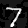
\includegraphics{../src/multirun/2025-08-30/22-19-32/0/fgsm_examples/adversarial_200_0_label_3.png}
        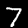
\includegraphics{../src/multirun/2025-08-30/22-19-32/0/fgsm_examples/original_200_0_label_7.png}
        \caption{Figure of a succesful adversarial attack with $\varepsilon=0.01$ on MNIST.
        The left is classified as a 3 while the right is the original image.}
        \label{fig:attack}
    \end{figure}

    \subsection{Generalized Gauss-Newton}
    The Gauss-Newton method is a classical optimization method, which was developed initially for least squares, but now have been adapted for neural networks.
    Rather than the usual SGD updates
    \begin{align*}
        \theta_{n+1} = \theta_n - \eta \nabla_{\theta} \mathcal L(x, \theta)
    \end{align*}
    where $\eta$ is the learning rate, generalized Gauss-Newton consists of using an approximation to the Hessian
    \begin{align*}
        \theta_{n+1} = \theta_n - \eta (\lambda I + J^THJ)^{-1} \nabla_{\theta} \mathcal L(x, \theta)
    \end{align*}
    where $J$ the Jacobian of the neural network, $H$ the Hessian of the loss with respect to the network, and $\lambda$ some positive regularizer.

    \subsection{Poisoned Dataset}

    \subsection{Loss Geometry and SAM analysis}


    \section{Methodology and analysis}
    We built and trained three different models using different optimizers: SGD, Adam and Gauss-Newton.
    While all three models have the exact same architecture and start with the same initial seeds, the use of different optimizers will result in them ending up with different behaviors.
    A simple, small CNN is chosen for sake of computational costs.
    These models are trained on the MNIST dataset, and a small grid search was conducted to find a candidate learning rate.
    This hyperparameter search is by no means exhaustive, especially for the Gauss-Newton case, where there are considerably more levers to tweak.
    All models are trained such that they achieve roughly 95\% accuracy on the test set.

    In a secondary experiment, we trained three additional models, one for each optimizer, on a ``poisoned`` dataset.
    This dataset was constructed by taking 10\% of the original training data and perturbing it with the wrong label.
    We refer the reader to the appendix or code base for the exact details.

    \subsection{Adversarial Robustness}
    With the models trained, all models are subject to adversarial attacks by FGSM.
    We perform a light sweep over the $\varepsilon$ parameter of \cref{eqn:fgsm} over $\{0.1, 0.05, 0.01\}$.
    In \Cref{tab:fgsm_results}, we show the results of the FGSM attacks on the clean dataset.
    It's clear that SGD and Adam have no discernible differences between the percentages, but Gauss-Newton results in a clear decrease in the number of succesful attacks.
    This trend is also seen in the poisoned dataset context.
    We show the results from the FGSM attack on the models trained on poisoned dataset in \cref{tab:fgsm_results_poisoned}.
    It seems that while Adam and SGD actually improved robustness, perhaps from being less prone to overfitting, Gauss-Newton did not significantly change at all.


    \begin{table}[ht!]
        \centering
        \caption{Performance of Models Under FGSM Attack for Varying Epsilon (Clean Data)}
        \label{tab:fgsm_results}
        \begin{tabular}{|l|c|c|c|c|}
            \hline
            \textbf{Optimizer} & \textbf{Correct Tests} & $\varepsilon=0.1$ & $\varepsilon=0.05$ & $\varepsilon=0.01$ \\
            \hline
            Adam               & 9778                   & 7396 (75.64\%)    & 3142 (32.13\%)     & 253 (2.59\%)       \\
            \hline
            SGD                & 9611                   & 7268 (75.62\%)    & 2687 (27.96\%)     & 227 (2.36\%)       \\
            \hline
            Gauss-Newton       & 9585                   & 4937 (51.51\%)    & 1334 (13.92\%)     & 159 (1.66\%)       \\
            \hline
        \end{tabular}
    \end{table}

    \begin{table}[ht!]
        \centering
        \caption{Performance of Models Under FGSM Attack for Varying Epsilon (Poisoned Data)}
        \label{tab:fgsm_results_poisoned}
        \begin{tabular}{|l|c|c|c|c|}
            \hline
            \textbf{Optimizer} & \textbf{Correct Tests} & $\varepsilon=0.1$ & $\varepsilon=0.05$ & $\varepsilon=0.01$ \\
            \hline
            Adam               & 9776                   & 6259 (64.02\%)    & 2105 (21.53\%)     & 186 (1.90\%)       \\
            \hline
            SGD                & 9553                   & 6016 (62.97\%)    & 1775 (18.58\%)     & 173 (1.81\%)       \\
            \hline
            Gauss-Newton       & 9581                   & 4888 (51.02\%)    & 1367 (14.27\%)     & 162 (1.69\%)       \\
            \hline
        \end{tabular}
    \end{table}

    \subsection{Simple Analysis}
    Beyond simple accuracy metrics, we sought to understand the geometric properties of the local minima that each optimizer converged to, and how these properties relate to adversarial robustness.
    We performed two key analyses to measure curvature.
    \subsubsection{Input Gradient Norm and Logit Margin Distributions}
    To understand the local geometry of the model's decision boundary in the input space, we measured the distribution of the input gradient norm and the logit margin for each model on the clean test set.

    The input gradient norm is defined as $\norm{\nabla_x \mathcal L(x, \theta)}^2$ the norm of the gradient at the loss.
    A high norm indicates that the model's output is highly sensitive to a small change in the input, suggesting that the data point is located in a region of high curvature.
    The common As such, a small perturbation can push an image into a different decision.
    We show the distribution over the test set in \cref{fig:grad-norm}.
    It's clear that Gauss-Newton's model resulted in a

    \begin{figure}
        \centering
        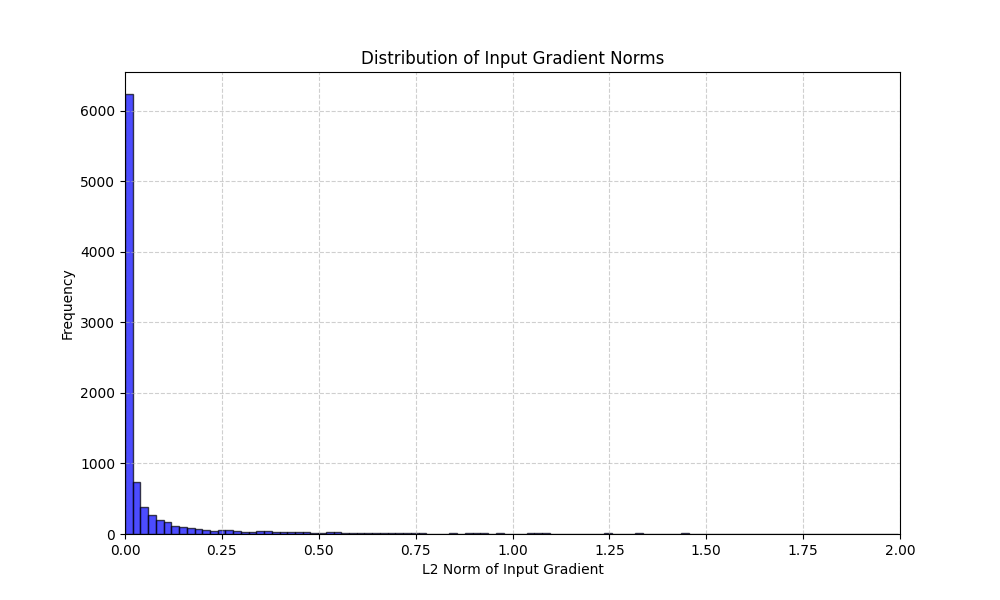
\includegraphics[width=0.4\textwidth]{../src/outputs/2025-09-10/23-05-38/input_gradient_norm_distribution.png}
        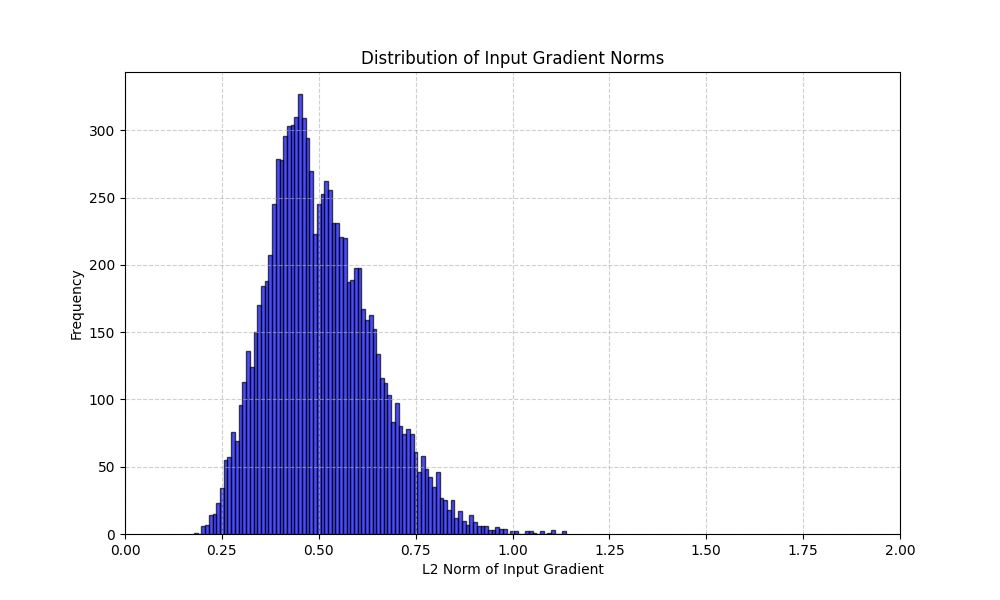
\includegraphics[width=0.4\textwidth]{../src/outputs/2025-09-10/23-05-59/input_gradient_norm_distribution.png}
        \caption{Figure of distribution of input gradient norms on the test set with Adam on the left and GN on right.
        Note that the Adam has significantly smaller norms, meaning the curvature near the model is more flat compared to GN.}
        \label{fig:grad-norm}
    \end{figure}

    \textbf{The Nature of Second-Order Optimization:}
    Your initial hypothesis was that Gauss-Newton's minimum might be different from SGD's.
    This finding confirms it. The Gauss-Newton optimizer, by using curvature information, may be converging to a minimum that is not as ``flat`` in the parameter space as an SGD minimum, but is in fact \textit{more robust} to input perturbations.
    This is a novel finding worth highlighting.
\end{document}